\documentclass[submit,techreq,noauthor]{ipsj}


\usepackage[dvipdfmx]{graphicx}
\usepackage{latexsym}

\def\Underline{\setbox0\hbox\bgroup\let\\\endUnderline}
\def\endUnderline{\vphantom{y}\egroup\smash{\underline{\box0}}\\}
\def\|{\verb|}

\begin{document}


\title{serverspec: 宣言的記述でサーバの状態をテスト可能な\\
汎用性の高いテストフレームワーク}

\paffiliate{PAPERBOY}{株式会社paperboy\&co.}

\paffiliate{TU}{帝京大学 理工学部情報科学科通信教育課程}

\paffiliate{KU}{京都大学 情報科学研究科,京都市\\
Graduates School of Infromatics, Kyoto University, Yoshida-Honmachi, Sakyo-ku, Kyoto-shi, 606-8501 Japan
}

\author{宮下 剛輔}{Miyashita Gosuke}{PAPERBOY,TU}[gosukenator@gmail.com]
\author{栗林 健太郎}{Kuribayashi Kentaro}{PAPERBOY}
\author{松本 亮介}{Matsumoto Ryosuke}{KU}

\begin{abstract}
システムの大規模・複雑化に伴い,サーバの構築・運用を効率化するために,サーバの状態をコードで記述する手法が数多く提案されている.それらの手法を効率良く扱うプロセスとして,テスト駆動開発の手法をサーバ構築に応用したTest-Driven Infrastructureが提案されている.このプロセスを支援するテストフレームワークもいくつか登場しているが,あるものは特定の構成管理ツールに依存,またあるものはOS毎の違いを自ら吸収しなければならないなど,汎用性に難がある.そこで,本論文では,特定の構成管理ツールやOSに依存することなく,サーバの状態を汎用的かつ可読性の高いコードでテスト可能なテストフレームワークを提案する.提案手法では,汎用性を高めるために,これまでのOSや構成管理ツール固有の振る舞いを整理して一般化し,汎用コマンド実行フレームワークとして定義する.これにより,運用業務で発生するコマンド群,特に確認作業に関して体系化・抽象化する.続いて,テストコード記述の抽象度を高め可読性を上げるために宣言的な記法で汎用コマンド実行フレームワークを操作できる制御テストフレームワークを定義する.これにより,管理者がOSや構成管理ツールの違いを気にすることなくサーバの状態を容易にテストできるようになり,サーバの運用・管理コストを低減できる.また,フレームワークを用途別に分離して定義することにより,制御テストフレームワークを独自の記述に変更する事も容易である.提案するテストフレームワークをserverspecと名付けた.
\end{abstract}


\maketitle

\section{はじめに}

科学やビジネス領域における問題の複雑化への要求へ応えるため,システムが大規模化・複雑化する\cite{survey_and_taxonomy_of_iaas}のに伴い,UNIXシェルにより書かれたプログラムに代わり,サーバの設定を宣言的なコードで扱う構成管理手法が提案された.その実装としてCFEngine\cite{cfengine}が登場した.その後様々な構成管理ツールが生み出されているが\cite{cmt},2005年のPuppetの登場\cite{puppet}と2006年のAmazon EC2の登場\cite{ec2}をきっかけに``Infrastructure as Code''という概念が台頭した.この概念における``Infrastructure''はアプリケーションを載せるためのインフラを意味し,OSやミドルウェアといったソフトウェアレイヤーを含む.そして,インフラをコードで扱うことから,アジャイルソフトウェア開発\cite{agile_manifesto}と同様の手法がサーバ構築・運用にも適用できるのでは,という発想が生まれ``Agile infrastructure and operations''\cite{agile_infrastructure}という流れが生じている.

``Agile infrastructures and operations''を実践するためのプロセスとして,テスト駆動開発\cite{test_driven_development}の手法をサーバ構築・運用に応用した``Test-Driven Infrastructure''\cite{test_driven_infrastructure_with_chef}というプロセスが提案されており,このプロセスを支援するテストフレームワークがいくつも登場している\cite{chefspec}\cite{rspec-puppet}\cite{cucumber-chef}\cite{minitest-chef-handler}\cite{test-kitchen}\cite{rspec-system}.これらのうち,ChefSpec\cite{chefspec},rspec-puppet\cite{rspec-puppet}は,構成管理ツール固有の言語で書かれたコードの内容をテストするのみで,実際にコードをサーバに適用した結果はテストしない.そのため,単体テストしては利用できるが結合テスト用途には利用できない.Cucumber-chef\cite{cucumber-chef},minitest-chef-handler\cite{minitest-chef-handler}はChefという特定の構成管理ツールに依存している.そのため,Chef以外の構成管理ツールでは利用することができない.Test Kitchen\cite{test-kitchen}やrspec-system\cite{rspec-system}は,テスト用VMの作成,テスト用VMへの構成管理ツールの適用,テストの実行をトータルで行う統合テストスイートであるが,組み込みのテスト機構は汎用性に乏しく,特定の構成管理ツールに依存していたり,OSやディストリビューション毎の違いを意識したテストコードを書く必要がある.

我々は,テストフレームワークの汎用性を高めるために,構成管理ツール特有の振る舞い,例えば,パッケージのインストールやシステムユーザの作成などを抽出,一般化し,それらをテストするためのコマンドをOSやディストリビューション毎に分離,その上でOSや実行形式の違いを吸収するレイヤーを設けることにより,汎用コマンド実行フレームワークを定義した.続いて,テストコードの記述の抽象度を高め可読性を上げるために,宣言的な記法で汎用コマンド実行フレームワークを操作できる制御テストフレームワークを定義した.これにより,テストコードのメンテナンス性を高め,サーバの運用・管理コストを低減することができる.また,フレームワークを用途別に分離して定義することにより,制御テストフレームワークを独自の記法に変更することも容易である.例えば,本論文で提案するテストフレームワークでは,テスト記法としてRSpec\cite{rspec}を採用しているが,minitest\cite{minitest}に差し替えたり,あるいはまったく独自の記法に差し替えたりすることも可能である.このテストフレームワークをserverspec\cite{serverspec}と名付けた.serverspecを採用している企業も既に存在する\cite{nintendo}\cite{wantedly}.

本論文の構成について述べる.2章ではサーバの構成管理とテスト手法について更に詳しく述べる.3章では提案するサーバのテスト手法と実装について述べ,4章では提案手法の評価について論じ,5章で結びとする.

\section{サーバの構成管理とテスト手法}

本論文で提案するストフレームワークは,サーバ構成を記述したコードのテストをいかに効率よく行うか,という観点から出発している.そこで代表的な構成管理ツールを例に,ツールと言語の特徴,テスト手法ならびに従来手法の問題点について言及する.

\subsection{CFEngineからChefへ}

安価なUNIXライクOSを搭載したサーバが普及し,TCP/IPにより異なるOSを搭載したサーバ同士がネットワーク接続可能になった.これによりシステムが大規模化・複雑化し,シェルスクリプトに代わり,サーバの設定を宣言的なコードで扱う構成管理手法が提案された.その実装としてCFEngine\cite{cfengine}が登場した.

2005年にはCFEngineに影響を受け発展させたPuppet\cite{puppet}が登場,2009年にはPuppetから影響を受けたChef\cite{chef}が登場している.CFEngine,Puppetは独自のDSL(Domain Specific Language)でサーバの構成を記述するが,ChefはRubyによる内部DSLで記述する.その特性ゆえ,Chefはシステム管理者よりも開発者に強く訴求し,Amazon EC2(Elastic Compute Cloud)の様な開発者自身がサーバ構築・運用を行える環境の普及とともに広まりを見せている.

\subsection{ChefからTest-Driven Infrastructureへ}

CFEngineやPuppetでは,記述できることが独自DSLの範囲内に収まるため,コードは比較的簡易なものとなる.しかしChefはRubyでできることはどんなことでも記述できる.そのためシステムが複雑になるにともない,それを記述するコードも複雑になる.そこでサーバ構成を記述したコードに対し,アジャイル開発におけるテスト駆動開発のプロセスを適用する事で,効率よくコードを記述することができる,といった考えが生まれる.Test-Driven Infrastuctureという概念はChefコミュニティ周辺で発生したものであるが,それは偶然ではなく,このようなChefが持つ言語特性ゆえである.

\subsection{Test-Driven Infrastructureにおけるテスト手法の分類}

Test-Driven Infrastructureにおけるテストの種類は,テスト駆動開発における以下の3つに分類できる.

\begin{enumerate}
  \item 単体テスト
  \item 結合テスト
  \item 受け入れテスト
\end{enumerate}

単体テストは構成管理ツールにおける``モジュール''に対するテストで,実際にコードをサーバに適用する前の段階で行うテストである.結合テストはコードをサーバに適用した後に行うテストで,コードが期待通りにサーバの設定を行ったかどうかをテストする.受け入れテストもコードをサーバに適用した後に行うテストだが,結合テストがサーバ内部の状態をテストするホワイトボックステストなのに対し,受け入れテストはサーバの外から見た振る舞いをテストするブラックボックステストであるという違いがある.

\subsection{従来テスト手法の問題点}

単体テストツールとしてはChefにはChefSpec,Puppetにはrspec-puppetというツールが存在する.その名が示すとおり,それぞれChefとPuppet専用のツールであり,単体テストツールとしては十分であるが,実際にコードをサーバに適用した結果をテストすることはできないため,単体テストツールだけでは不十分である.

結合テストツールとしては,minitest-chef-handler,Test Kitchen,rspec-systemが存在する.この内minitest-chef-handlerとTest KitchenはChefに依存したツールであり,他の構成管理ツールとともに利用することができない.Test Kitchenやrspec-systemは,テスト用VMの作成,テスト用VMへの構成管理ツールの適用,テストの実行をトータルで行う統合テストスイートであるが,ツール標準のテスト機構は汎用性に乏しく,特定の構成管理ツールに依存していたり,OSやディストリビューション毎の違いを意識したテストコードを書く必要がある.

受け入れテストツールとしてはcucumber-chef,leibnizが存在するが,これらはChefに依存したツールであり,他の構成管理ツールとともに利用することができない.

以上をまとめると表\ref{tab:comparison}のようになる.

\begin{table}[htb]
  \begin{center}
    \begin{tabular}{|c|c|c|c|}
      \hline
      ツール名 & テスト種別 & ツール独立性 & OS汎用性 \\
      \hline
      \hline
      ChefSpec              & 単体 & ×  & ○ \\
      \hline
      rspec-puppet          & 単体 & ×  & ○ \\
      \hline
      minitest-chef-handler & 結合 & ×  & ○ \\
      \hline
      Test Kitchen          & 結合 & ×  & × \\
      \hline
      rspec-system          & 結合 & ○ & × \\
      \hline
      Cucumber-Chef         & 受入 & ×  & ○ \\
      \hline
      leibniz               & 受入 & ×  & ○ \\
      \hline
    \end{tabular}
    \label{tab:comparison}
    \caption{テストツール比較表}
  \end{center}
\end{table}



\section{提案するサーバテスト手法}

構成管理ツール独立性とOS・ディストリビューション汎用性をいかに満たすかを考察する.

特定の構成管理ツールからの独立性を満たせない理由は2つある.ひとつは構成管理ツールがもつOS・ディストリビューション汎用性を利用するために,テストの実装が特定の構成管理ツールに依存していることである.

もうひとつはテストスイートでのテスト用VM構築フェーズが,特定の構成管理ツールのみ対応していることである.

OS・ディストリビューション汎用性が満たせないのは,テストがシェルコマンドを直接記述する実装になっており,OS・ディストリビューションの違いをテストコードを書く者自らが意識しないといけないからである.

この考察から,提案するテスト手法に必要な要件は以下の通りとなる.

\begin{enumerate}
  \item テストの実装を特定の構成管理ツールに依存しない
  \item テストスイートではなくテストのみに特化する
  \item OS・ディストリビューションの違いを利用者に意識させない
\end{enumerate}

そこでまずOS・ディストリビューション毎にコマンドを分離し,統一的なAPIでコマンドを呼び出すことができる汎用コマンド実行フレームワークを定義する.このフレームワークではまず構成管理ツール固有の振る舞い(パッケージインストール等)を抽出する.そして振る舞いをテストするためのAPIを定義する.更にAPIから呼び出されるコマンドをOS・ディストリビューション毎に定義する.APIとコマンド群の間にはOS・ディストリビューションを判別して自動で適したコマンドを返すレイヤーを設ける.これにより運用業務で発生するコマンド群,特に確認作業に必要なコマンド群の体系化・抽象化を行う.

次に,テストコードの記述の抽象性を高め可読性を上げるために,宣言的な記法で汎用コマンド実行フレームワークを操作できる制御テストフレームワークを定義する.このフレームワークではまず記法の定義を行う.次に記法内の各命令と実際に呼び出す汎用コマンド実行フレームワークのAPIメソッドをひもづける.

汎用コマンド実行フレームワークと制御テストフレームワークの仕組みおよびその関係を\figref{fig:framework}に示す.

\begin{figure}[tb]
  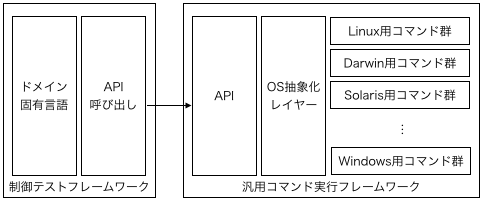
\includegraphics{framework-overview.png}
  \caption{汎用コマンド実行フレームワークと制御テストフレームワークの仕組みと関係}
  \label{fig:framework}
\end{figure}

この手法に基づき実装した汎用コマンド実行フレームワークをSpecInfra\cite{specinfra},制御テストフレームワークをserverspec\cite{serverspec}と名付けた.

SpecInfraとserverspecの実装の一部を示す.SpecInfraでは各OS用のコマンド群をクラスとして定義する.例としてRedHat系Linux上で指定されたパッケージがインストールされているかどうかを確認するコマンドの定義を\figref{fig:check-installed-on-redhat}に示す.また,Solaris上で指定されたパッケージがインストールされているかどうかを確認するコマンドの定義を\figref{fig:check-installed-on-solaris}に示す.serverspec上でこのコマンドを呼び出して指定したパッケージがインストールされているかどうかテストする部分の実装を\figref{fig:call-check-install}に示す.

\begin{figure}[tb]
\setbox0\vbox{
\begin{verbatim}
module SpecInfra::Command
  class RedHat < Linux
    def check_installed(package,version=nil)
      cmd = "rpm -q #{escape(package)}"
      if version
        cmd = "#{cmd} | grep -w -- #{escape(version)}"
      end
      cmd
    end
  end
end
\end{verbatim}
}
\centerline{\fbox{\box0}}
\caption{パッケージがインストールされているかを確認するRedHat系Linux用コマンド定義\label{fig:check-installed-on-redhat}}
\end{figure}

\begin{figure}[tb]
\setbox0\vbox{
\begin{verbatim}
module SpecInfra::Command
  class Solaris < Base
    def check_installed(package, version=nil)
      cmd = "pkg list -H #{escape(package)}"
      if version
        cmd = "#{cmd} | grep -qw -- #{escape(version)}"
      end
      cmd
    end
  end
end
\end{verbatim}
}
\centerline{\fbox{\box0}}
\caption{パッケージがインストールされているかを確認するSolaris用コマンド定義\label{fig:check-installed-on-solaris}}
\end{figure}


\begin{figure}[tb]
\setbox0\vbox{
\begin{verbatim}
module Serverspec::Type
  class Package < Base
    def installed?(provider, version)
      backend.check_installed(@name, version)
    end
  end
end
\end{verbatim}
}
\centerline{\fbox{\box0}}
\caption{パッケージインストールチェックコマンドを呼び出す部分のservespecでの実装\label{fig:call-check-install}}
\end{figure}

これらの実装の上で,サーバ上にntpパッケージがインストールされているかどうかを確認するためのテストコードをserverspecの記法で記述したものを\figref{fig:test-code-to-check-ntp-package-installed}に示す.

\begin{figure}[tb]
\setbox0\vbox{
\begin{verbatim}
describe package("ntp") do
  it { should be_installed }
end
\end{verbatim}
}
\centerline{\fbox{\box0}}
\caption{ntpパッケージがインストールされているかをテストするserverspecで記述したテストコード\label{fig:test-code-to-check-ntp-package-installed}}
\end{figure}

\section{提案手法の評価}

Test Kitchen標準のbats\cite{bats}によるテストコードとserverspecのテストコードを比較し評価する.

batsによるUbuntu\cite{ubuntu}上でのテストコードを\figref{fig:test-with-bats-on-ubuntu}に示す.また,同じ内容のテストをSolaris\cite{solaris}向けに書く場合の例を\figref{fig:test-with-bats-on-solaris}に示す.serverspecによるテストコードは,OSが何であっても\figref{fig:test-with-serverspec}で示すようなコードになる.このように,提案手法ではOSの違いを意識することなく,テストコードを記述することができる.

\begin{figure}[tb]
\setbox0\vbox{
\begin{verbatim}
@test "The package apache2 is installed" {
  dpkg-query -f '${Status}' -W apache2 \
    | grep '^install ok installed$'
}

@test "The apache2 service is running" {
  service apache2 status
}

@test "Port 80 is listening" {
  netstat -tunl | grep ":80 "
}
\end{verbatim}
}
\centerline{\fbox{\box0}}
\caption{batsによるUbuntu上でのテストコード\label{fig:test-with-bats-on-ubuntu}}
\end{figure}

\begin{figure}[tb]
\setbox0\vbox{
\begin{verbatim}
@test "The package apache2 is installed" {
  pkg list -H apache2
}
 
@test "The apache2 service is running" {
  svcs -l apache2 | egrep '^status *online$'
}
 
@test "Port 80 is listening" {
  netstat -an | grep LISTEN | grep ".80 "
}
\end{verbatim}
}
\centerline{\fbox{\box0}}
\caption{batsによるSolaris上でのテストコード\label{fig:test-with-bats-on-solaris}}
\end{figure}

\begin{figure}[tb]
\setbox0\vbox{
\begin{verbatim}
describe package("apache2") do
  it { should be_installed }
end
 
describe service("apache2") do
  it { should be_running }
end
 
describe port(80) do
  it { should be_listning }
end
\end{verbatim}
}
\centerline{\fbox{\box0}}
\caption{serverspecによるテストコード\label{fig:test-with-serverspec}}
\end{figure}

\begin{figure}[tb]
\setbox0\vbox{
\begin{verbatim}
@test "/etc/sudoers is not readable by others" {
  ls -l /etc/sudoers | egrep '^......-..'
}
\end{verbatim}
}
\centerline{\fbox{\box0}}
\caption{batsによる/etc/sudoersが他人から読めないことをテストするコード\label{fig:test-permission-with-bats}}
\end{figure}

\begin{figure}[tb]
\setbox0\vbox{
\begin{verbatim}
describe file("/etc/sudoers") do
  it { should_not be_readable.by("others") }
end
\end{verbatim}
}
\centerline{\fbox{\box0}}
\caption{serverspecによる/etc/sudoersが他人から読めないことをテストするコード\label{fig:test-permission-with-serverspec}}
\end{figure}

別の比較として,/etc/sudoersが他人から読めないことをテストするコードの例を示す.batsでは\figref{fig:test-permission-with-bats}に示すコードとなり,serverspecでは\figref{fig:test-permission-with-serverspec}に示すコードとなる.このように, batsはテストコードだけでは何をテストしているのか判別しにくいため,説明用のテキストが必要となる.一方serverspecはテストコードだけでテスト内容が理解できるため,別途説明用のテキストを必要としない.

serverspecはオープンソースで公開されており,上述のような利用ための敷居の低さ,単機能,記法の汎用性・抽象度の高さから,利用が広がっている.また,採用している企業もいくつか見受けられる\cite{nintendo}\cite{wantedly}.しかし,定量的な評価ができておらず,評価手法の検討など,今後に課題が残る.

\section{まとめ}

本論文では,Test-Driven Infrastructureを支援するための従来テストフレームワーク手法の問題点について指摘し,解決するために必要な要件として,構成管理ツール独立性とOS・ディストリビューション汎用性を提案した.また,これらの要件を満たすために,汎用コマンド実行フレームワークと制御テストフレームワークに分離して定義する手法についても提案した.これらふたつの実装例としてSpecInfraとserverspecを紹介した.

serverspecの登場によってTest-Driven Infrastuctureというプロセスが国内でも徐々に認知され,この分野の今後の発展が期待される.またSpecInfraを基盤としたserverspecよりも優れた実装の登場や,多種ツールへのSpecInfraの応用(例えば構成管理ツールなど)も今後期待される.

今後の課題として,提案手法による運用効率の向上の定量的評価ができていないので,評価手法について検討するとともに,手法に関する助言を募りたい.




\begin{thebibliography}{99}

\bibitem{cfengine}
Mark Burgess, ``CFEngine: a system configuration engine'',
University of Oslo report 1993,
http://cfengine.com/markburgess/papers/cfengine\_history.pdf

\bibitem{cmt}
``Comparison of open-source configuration management software'',
http://en.wikipedia.org/wiki/Comparison\_of\_open\_source\_configuration\_management\_software.

\bibitem{puppet}
Luke Kanies,
``Puppet: Next-Generation Configuration Management'',
USENIX ;login, February 2006, Volume 31, Number 1
https://c59951.ssl.cf2.rackcdn.com/807-kanies\_0.pdf.

\bibitem{ec2}
``Release: Amazon EC2 on 2006-08-23'',
http://aws.amazon.com/releasenotes/Amazon-EC2/353.

\bibitem{agile manifesto}
``アジャイルソフトウェア開発宣言'',
http://agilemanifesto.org/iso/ja/.

\bibitem{agile infrastructure}
Patrick Debois,
``Agile infrastructure and operations: how infra-gile are you?'',
Agile, 2008. AGILE '08. Conference,
http://www.jedi.be/presentations/IEEE-Agile-Infrastructure.pdf.

\bibitem{test driven development}
Kent Beck,
``Test Driven Development: By Example'',
ISBN: 978-0321146533.

\bibitem{test driven infrastructure with chef}
Stephen Nelson-Smith,
``Test-Driven Infrastructure with Chef, 2nd Edition
Bring Behavior-Driven Development to Infrastructure as Code'',
ISBN: 978-1449372200.

\bibitem{chefspec}
``ChefSpec'', http://code.sethvargo.com/chefspec/.

\bibitem{rspec-puppet}
``rspec-puppet'', http://rspec-puppet.com/.

\bibitem{cucumber-chef}
``Cucumber-Chef'', http://www.cucumber-chef.org/.

\bibitem{minitest-chef-handler}
``minitest-chef-handler'', https://github.com/calavera/minitest-chef-handler.

\bibitem{test kitchen}
``Test Kitchen'', http://kitchen.ci/.

\bibitem{rspec-system}
``rspec-system'', https://github.com/puppetlabs/rspec-system.

\bibitem{rspec}
``RSpec``, http://rspec.info/.

\bibitem{minitest}
``minitest'', http://docs.seattlerb.org/minitest/.

\bibitem{serverspec}
``serverspec'', https://github.com/serverspec/serverspec.

\bibitem{nintendo}
``採用情報:キャリア採用 募集要項 - 京都勤務の募集職種 開発部門'',
http://www.nintendo.co.jp/jobs/career/kyoto\_sec1.html\#p03.

\bibitem{wantedly}
serverspecの求人 - Wantedly,
https://www.wantedly.com/projects/search?utf8=%E2%9C%93&q=serverspec.

\bibitem{chef}
``Chef - Code Can | Chef'', http://www.getchef.com/.

\bibitem{ec2}
``Amazon Elastic Compute Cloud'',
http://aws.amazon.com/jp/ec2/.

\bibitem{ruby}
``オブジェクト指向スクリプト言語 Ruby'',
https://www.ruby-lang.org/ja/.

\bibitem{specinfra}
``specinfra'', https://github.com/serverspec/specinfra.

\bibitem{busser-serverspec}
``cl-lab-k/busser-serverspec'',
https://github.com/cl-lab-k/busser-serverspec.

\bibitem{rspec-system-serverspec}
``puppetlabs/rspec-system-serverspec'',
https://github.com/puppetlabs/rspec-system-serverspec.

\bibitem{vagrant}
``Vagrant'',
http://www.vagrantup.com/.

\bibitem{vagrant-serverspec}
``jboorhis/vagrant-servers@ec'',
https://github.com/jvoorhis/vagrant-serverspec.

\bibitem{bats}
``sstephenson/bats'',
https://github.com/sstephenson/bats.

\bibitem{ubuntu}
``The world's most popular free OS | Ubuntu'',
http://www.ubuntu.com/.

\bibitem{solaris}
``Oracle Solaris'',
http://www.oracle.com/jp/products/servers-storage/solaris/overview/index.html.

\end{thebibliography}


\end{document}
